
\section{Theorie}
\label{sec:Theorie}
Um die Natur der Elektronenhülle zu untersuchen werden Elektronenstöße untersucht.
Hierzu werden Atome mit Elektronen beschossen. Aus den auftretenden Energieverlusten
lässt sich anschließend auf die Natur der Elektronen schließen. Auch der Frank-Hertz
Versuch, bei welchem Hg-Atome verwendet werden,
folgt diesem Konzept. Es treten nun sowohl elastische als auch unelastische Stöße auf.
Für letztere folgt bei nicht relativistischen Betrachtung der Energieunterschied:
\begin{equation}
  m_0 \frac{v_\text{vor}²}{2} - m_0 \frac{v_\text{nach}²}{2} = \Delta E = E_1 - E_0\label{eq:Estoss}
  \end{equation}
Die auftretende Energiedifferenz $\Delta E$ wird dazu verwendet, das beschossene
Atom von seinem Grundzustand $E_0$ in den angeregten Zustand $E_1$ anzuheben. Kurz
darauf fällt es wieder in den Grundzustand zurück und emittiert dabei einen Lichtquant der Frequenz
\begin{equation}
  f = \frac{\Delta E}{h} \label{eq:f}
  \end{equation}

  \begin{figure}
 \centering
 \caption{Der prinzipielle Aufbau des Frank-Hertz-Versuches.}
 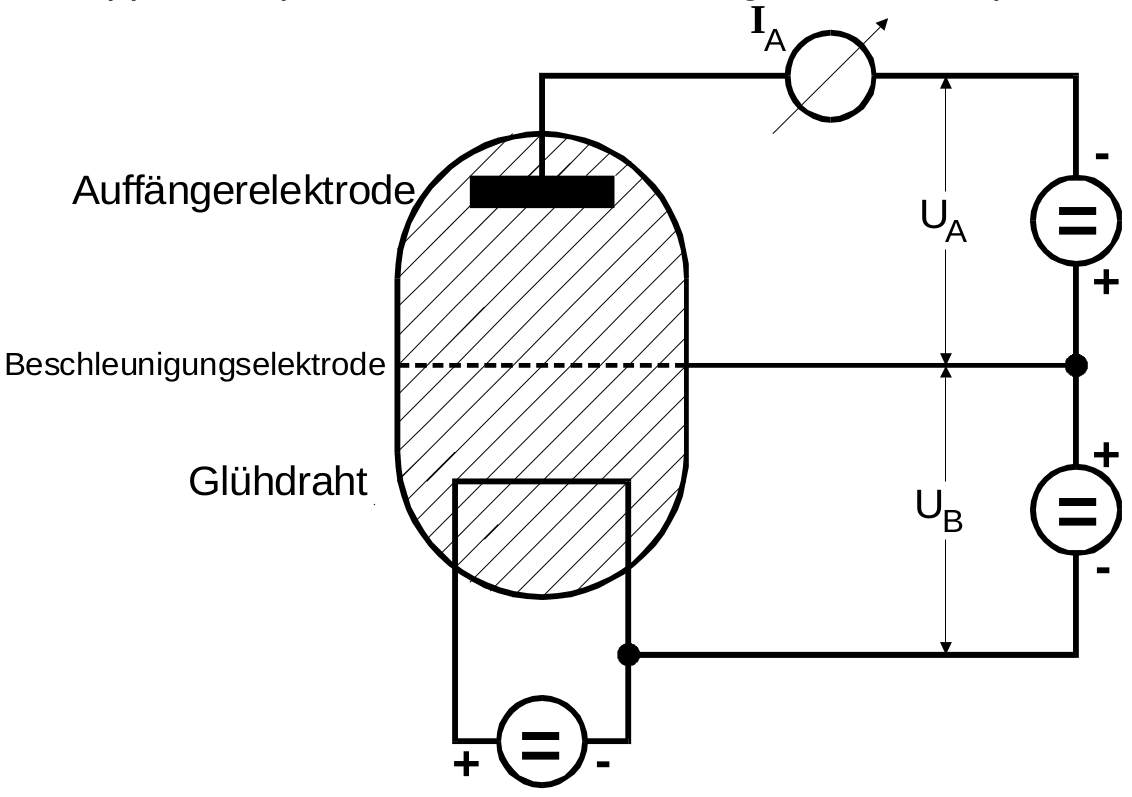
\includegraphics[width=\linewidth-170pt,height=\textheight-170pt,keepaspectratio]{content/franktheorie.png}
 \label{fig:franktheorie}
\end{figure}

Der theoretische Aufbau des Frank-Hertz Versuches nach Abb.
\ref{fig:franktheorie} . Den Kern bildet eine mit Quecksilberdampf versehene und ansonsten evakuierte
Röhre. Elektronen werden mithilfe einer Glühspannung aus einer Glühkathode emittiert
und mittels einer Beschleunigungsspannung bis zu einer in der Mitte angebrachten
Elektrode beschleunigt. Die Elektronen haben danach die Energie
\begin{equation}
  m_0 \frac{v_\text{vor}²}{2} = e_0 U_\text{B}\text{.}\label{eq:ekin}
  \end{equation}
   Anschließend werden die Elektronen mit einer Auffängerelektrode
gefangen und der daraus resultierende Strom gemessen.
Bei Variation von $U_\text{B}$ ergibt sich daher den bohrschen Postulaten nach eine
 Kurve wie in Abb. \ref{fig:Graphtheorie}. Zunächst passiert nichts, bis $U_\text{B}$ größer als $U_\text{A}$ ist.
 Dann lässt sich ein Anstieg der Stromstärke beobachten, bis die kinetische Energie
 der Elektronen $\Delta E$ erreicht. Nun treten unelastische Stöße auf und die Elektronen
 verlieren ihre kinetische Energie, sodass sie die Auffängeranode nicht mehr erreichen.
 Infolgedessen folgt einer plötzliches absinken der Stromstärke auf 0.  Bei höheren
 Spannungen können die Elektronen wieder schnell genug beschleunigen, sodass der
 Vorgang mehrfach durchlaufen wird. Für den Spannungsabstand zwischen 2 Maxima folgt daher:
 \begin{equation}
   U_1 = \frac{1}{e_0}\left( E_1 - E_0 \right)\label{eq:udiff}
   \end{equation}


   \begin{figure}
   	\centering
   	\caption{Der theoretische Verlauf der Frank-Hertz-Kurve.}
   	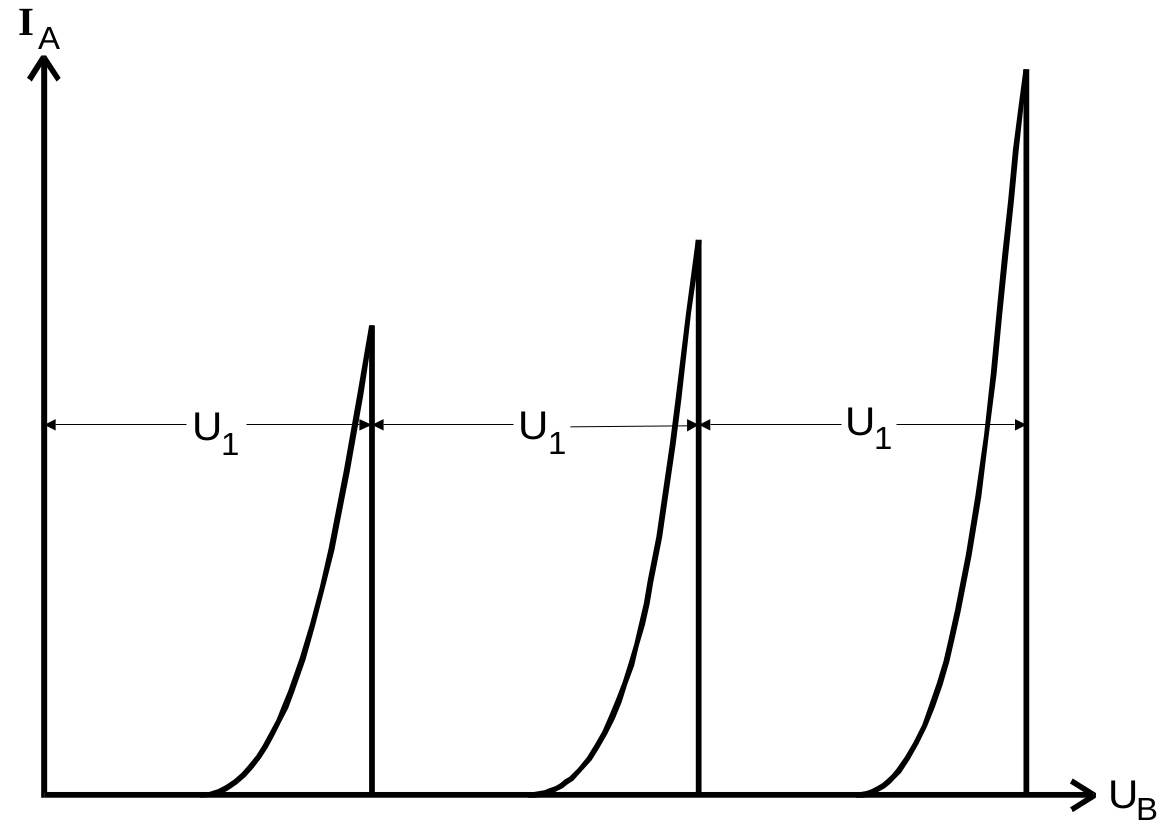
\includegraphics[width=\linewidth-170pt,height=\textheight-170pt,keepaspectratio]{content/theorie.png}
   	\label{fig:Graphtheorie}
   \end{figure}



Der in Abb. \ref{fig:Graphtheorie} dargestellte idealisierte Kurvenverlauf wird jedoch
aufgrund mehrerer Faktoren nicht erreicht.


\begin{itemize}
  \item \subsection{Die Auswirkungen des Kontaktpotentials}
  Wenn die Materialien der Glühkathode und der Beschleunigungselektrode unterschiedliche
  Austrittsarbeiten besitzen verschiebt sich das effektive $U_\text{B}$ bezüglich
  eingestellten. Um jedoch bereits bei niedrigen Temperaturen hohe Emissionsrate
  zu erreichen, besitzt die Glühkathode ein Material mit geringer Austrittsarbeit $\Phi_\text{G}$.
  Damit es jedoch zu keiner Verfälschung der Daten durch austretende Elektronen an
  der Beschleunigungselektrode besitzt dessen Material eine weitaus größere Austrittsarbeit
  $\Phi_\text{B}$. Daher ergibt sich eine effektives Beschleunigungspotential durch
  \begin{equation}
    U_\text{B,eff} = U_\text{B} - K \text{ mit dem Kontaktpotential }K\text{, } K = \frac{1}{e_0}\left(\Phi_\text{B} - \Phi _\text{G} \right)\text{, }\label{eq:kontakt}
  \end{equation}
was sich in einer Verschiebung der Kurve um $K$ widerspiegelt.

\item \subsection{Das Energiespektrum der Elektronen}
Des weiteren besitzen die Elektronen im Kathodenmaterial keine feste Energie, sondern
verteilen sich gemäß der Fermi-Dirac-Verteilung. Daher treten die Elektronen mit
unterschiedlichen Anfangsgeschwindigkeiten aus. Die zu beobachteten unelastischen Stöße treten
daher nicht mehr an einer fest definierten Stelle auf, sondern auf einem Bereich.
Infolgedessen fallen die Extrema geringer aus und der Graph fällt nach einem
Maximum nicht mehr unstetig auf 0, sondern nähert sich dieser nur noch an. Zusätzlich
ist der Einfluss der elastischen Stöße zu berücksichtigen. Da der gemessene
Strom auschließlich von der Geschwindigkeitskomponente in Normalrichtung bezüglich
der Anode abhängt, wird die Kurve durch elastische Stöße im Auffangbereich verändert,
da weniger Elektronen das Gegenfeld durchlaufen. Die Frank-Hertz-Kurve wird daher flacher und breiter.


\item\subsection{Die Auswirkungen des Dampfdruckes}
Damit es zu einer geeigneten Anzahl von Zusammenstößen zwischen Elektronen und Hg-Atomen
kommt muss die mittlere freie Weglänge $\overline{w}$ der Hg-Atome klein gegenüber
der Beschleunigungsstrecke sein. Diese hängt vom vorherrschenden , temperaturabhängigen
Sättigungsdampfdruck $p_\text{sät}$ ab. Damit folgt
%mit der Dampfdruckkurve in Abb. \ref{fig:Graphdampf}
die Näherung:
\begin{equation}
  \overline{w} [cm] = \frac{0.0029}{5.5 \cdot 10⁷} \exp \left(\frac{-6876}{T}\right)\text{,}\label{eq:w}
  \end{equation}
  mit der Temperatur $T$ in Kelvin. Ist $\overline{w}$ zu groß, wächst die Wahrscheinlichkeit,
  dass Elektronen den Beschleunigungsbereich ohne Wechselwirkung durchlaufen. Ist
  $p_\text{sät}$ zu groß, treten zu viele elastische Stöße auf, welche das Ergebnis
  wie bereits beschrieben, verfälschen.
\end{itemize}

%\begin{figure}
% \centering
 %\caption{Der Verlauf der Dampdruckkurve für Hg.}
 %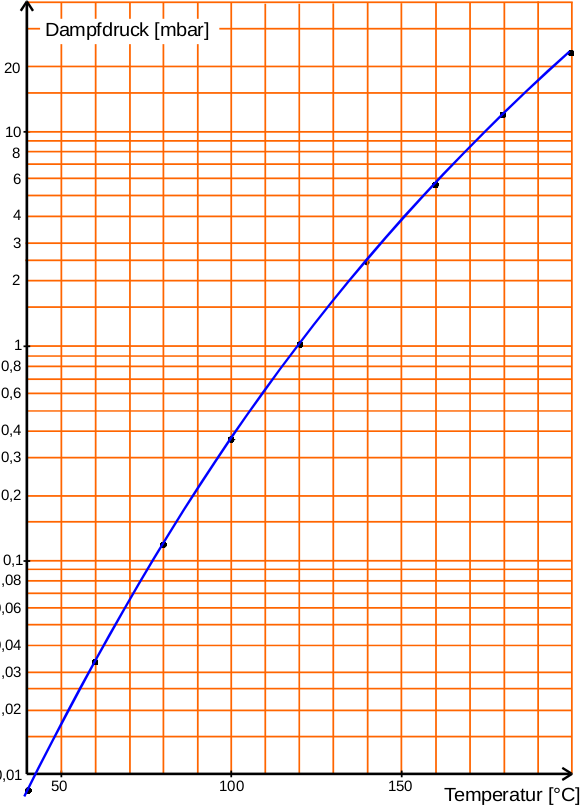
\includegraphics[width=\linewidth-170pt,height=\textheight-170pt,keepaspectratio]{content/dampf.png}
 %\label{fig:Graphdampf}
%\end{figure}
